\documentclass[11pt]{article}\usepackage[]{graphicx}\usepackage[usenames,dvipsnames]{xcolor}
% maxwidth is the original width if it is less than linewidth
% otherwise use linewidth (to make sure the graphics do not exceed the margin)
\makeatletter
\def\maxwidth{ %
  \ifdim\Gin@nat@width>\linewidth
    \linewidth
  \else
    \Gin@nat@width
  \fi
}
\makeatother

\definecolor{fgcolor}{rgb}{0.345, 0.345, 0.345}
\newcommand{\hlnum}[1]{\textcolor[rgb]{0.686,0.059,0.569}{#1}}%
\newcommand{\hlstr}[1]{\textcolor[rgb]{0.192,0.494,0.8}{#1}}%
\newcommand{\hlcom}[1]{\textcolor[rgb]{0.678,0.584,0.686}{\textit{#1}}}%
\newcommand{\hlopt}[1]{\textcolor[rgb]{0,0,0}{#1}}%
\newcommand{\hlstd}[1]{\textcolor[rgb]{0.345,0.345,0.345}{#1}}%
\newcommand{\hlkwa}[1]{\textcolor[rgb]{0.161,0.373,0.58}{\textbf{#1}}}%
\newcommand{\hlkwb}[1]{\textcolor[rgb]{0.69,0.353,0.396}{#1}}%
\newcommand{\hlkwc}[1]{\textcolor[rgb]{0.333,0.667,0.333}{#1}}%
\newcommand{\hlkwd}[1]{\textcolor[rgb]{0.737,0.353,0.396}{\textbf{#1}}}%
\let\hlipl\hlkwb

\usepackage{framed}
\makeatletter
\newenvironment{kframe}{%
 \def\at@end@of@kframe{}%
 \ifinner\ifhmode%
  \def\at@end@of@kframe{\end{minipage}}%
  \begin{minipage}{\columnwidth}%
 \fi\fi%
 \def\FrameCommand##1{\hskip\@totalleftmargin \hskip-\fboxsep
 \colorbox{shadecolor}{##1}\hskip-\fboxsep
     % There is no \\@totalrightmargin, so:
     \hskip-\linewidth \hskip-\@totalleftmargin \hskip\columnwidth}%
 \MakeFramed {\advance\hsize-\width
   \@totalleftmargin\z@ \linewidth\hsize
   \@setminipage}}%
 {\par\unskip\endMakeFramed%
 \at@end@of@kframe}
\makeatother

\definecolor{shadecolor}{rgb}{.97, .97, .97}
\definecolor{messagecolor}{rgb}{0, 0, 0}
\definecolor{warningcolor}{rgb}{1, 0, 1}
\definecolor{errorcolor}{rgb}{1, 0, 0}
\newenvironment{knitrout}{}{} % an empty environment to be redefined in TeX

\usepackage{alltt}
\usepackage[sc]{mathpazo} %Like Palatino with extensive math support
\usepackage{fullpage}
\usepackage[authoryear,sectionbib,sort]{natbib}
\linespread{1.7}
\usepackage[utf8]{inputenc}
\usepackage{lineno}
\usepackage{titlesec}
\titleformat{\section}[block]{\Large\bfseries\filcenter}{\thesection}{1em}{}
\titleformat{\subsection}[block]{\Large\itshape\filcenter}{\thesubsection}{1em}{}
\titleformat{\subsubsection}[block]{\large\itshape}{\thesubsubsection}{1em}{}
\titleformat{\paragraph}[runin]{\itshape}{\theparagraph}{1em}{}[. ]\renewcommand{\refname}{Literature Cited}
% my addnl packages
\usepackage{geometry}
\usepackage{graphicx}
\usepackage[T1]{fontenc}
\usepackage[utf8]{inputenc}
\usepackage{authblk}
\usepackage{setspace}
\usepackage{amsfonts,amssymb,amsmath,hyperref}
\usepackage{float}
\usepackage{caption}
\usepackage{multirow}
\usepackage{hyperref}
\usepackage{wrapfig}
\usepackage{rotating}
\usepackage[usenames,dvipsnames]{xcolor}

\newcommand{\tom}[2]{{\color{red}{#1}}\footnote{\textit{\color{red}{#2}}}}

\doublespacing
%\bibliography{creosote_SIPM}



%-------------------------------------------------------------------------

\title{Is shrub expansion into grasslands pushed or pulled? A spatial integral projection model for woody plant encroachment}

\author[a]{Trevor Drees}
\author[b]{Brad M. Ochocki}
\author[c]{Scott L. Collins}
\author[b]{Tom E.X. Miller$^{\ast}$}
\affil[a]{Department of Biology, Penn State University, State College, PA USA}
\affil[b]{Program in Ecology and Evolutionary Biology, Department of BioSciences, Rice University, Houston, TX USA}
\affil[c]{Department of Biology, University of New Mexico, Albuquerque, NM USA}

%-------------------------------------------------------------------------
\IfFileExists{upquote.sty}{\usepackage{upquote}}{}
\begin{document}
\maketitle
\noindent{} $\ast$ Corresponding author: tom.miller@rice.edu\\
\noindent{} Submitted to \textit{Ecological Monographs}\\
\noindent{} Manuscript type: Article\\
\noindent{} Open Research statement: All of our data and code are available during peer review at \url{https://github.com/TrevorHD/LTEncroachment}. This manuscript and its contents can be reproduced from this file: \url{https://github.com/TrevorHD/LTEncroachment/blob/master/Manuscript/creosote_SIPM_EcologicalMonographs_submission1.Rnw}. Upon acceptance, all data will be provided via creation and publication of an Environmental Data Initiative (EDI) data package, and code will be archived via Zenodo.
%\SweaveOpts{concordance=TRUE}

\linenumbers

%-------------------------------------------------------------------------
\newpage
\section*{Abstract}
The encroachment of woody plants into grasslands is a global phenomenon with implications for biodiversity and ecosystem function. 
Understanding and predicting the pace of expansion and the underlying processes that control it are key challenges in the study and management of woody encroachment.
Theory from spatial population biology predicts that the occurrence and speed of population expansion should depend sensitively on the nature of conspecific density dependence.
If fitness is maximized at the low-density encroachment edge then shrub expansion should be ``pulled'' forward.
However, encroaching shrubs have been shown to exhibit positive feedbacks, whereby shrub establishment modifies the environment in ways that facilitate further shrub recruitment and survival. 
In this case there may be a fitness cost to shrubs at low density causing expansion to be ``pushed'' from behind the leading edge.
We studied the spatial dynamics of creosotebush (\textit{Larrea tridentata}), which has a history of encroachment into Chihuahuan Desert grasslands over the past century.
We used observational data and seedling transplant experiments to test the strength and direction of density dependence in shrub demographic performance along a gradient of shrub density at the grass-shrub ecotone. 
We also used seed-drop experiments and wind data to construct a mechanistic seed dispersal kernel, then connected demography and dispersal data within a spatial integral projection model (SIPM) to predict the dynamics of shrub expansion.
The SIPM predicted that, contrary to expectations based on potential for positive feedbacks, the shrub encroachment wave is ``pulled'' by maximum fitness at the low-density front.
However, the predicted pace of expansion was strikingly slow (ca. 8 cm/yr), and this prediction was supported by independent re-surveys of the ecotone showing little to no change in spatial extent of shrub cover over 12 years. 
Encroachment speed was acutely sensitive to seedling recruitment, suggesting that this population may be primed for pulses of expansion under conditions that are favorable for recruitment.
Our integration of observations, experiments, and modeling reveals not only that this ecotone is effectively stalled under current conditions, but also \emph{why} that is so and how that may change as the environment changes. 

%-------------------------------------------------------------------------
\section*{Keywords}

density-dependence, ecotones, woody encroachment, shrubs, integral projection model, dispersal, Allee effects

%--------------------------------------------------------------------
\newpage
\section*{Introduction}
The recent and ongoing encroachment of shrubs and other woody plants into adjacent grasslands has caused significant vegetation changes across arid and semi-arid landscapes worldwide \citep{van2000shrub, van2009causes, goslee2003high, gibbens2005vegetation,parizek2002soil, cabral2003shrub,trollope1989encroachment, roques2001dynamics}.
The process of encroachment generally involves increases in the number or density of woody plants in both time and space \citep{van2000shrub}, which can drive shifts in plant community structure and alter ecosystem processes \citep{schlesinger1990biological, ravi2009can,schlesinger1998plant, knapp2008shrub}.
Other effects of encroachment include changes in ecosystem services \citep{reed2015reorienting, kelleway2017review}, declines in biodiversity \citep{ratajczak2012woody, sirami2012changes, brandt2013regime}, and economic losses in areas where the proliferation of shrubs adversely affects grazing land and pastoral production \citep{mugasi2000economic, oba2000bush}.

Woody plant encroachment can be studied through the lens of spatial population biology as a wave of individuals that may expand across space and over time \citep{kot1996dispersal, neubert2000demography, wang2002integrodifference, pan2012invasion}.
Theory predicts that the speed of wave expansion depends on two processes: local demography and dispersal of propagules.
First, local demographic processes include recruitment, survival, growth, and reproduction, which collectively determine the rate at which newly colonized locations increase in density and produce new propagules. 
Second, colonization events are driven by the spatial dispersal of propagules, which is commonly summarized as a probability distribution of dispersal distances, or ``dispersal kernel''.
The speed at which expansion waves move is highly dependent upon the shape of the dispersal kernel and can be strongly influenced by long-distance dispersal events in the tail of the distribution \citep{skarpaas2007dispersal}.
Both demography and dispersal may depend on plant size, since larger plants often have improved demographic performance and release seeds from greater heights, leading to longer dispersal distances \citep{nathan2011mechanistic}.
Accounting for population structure, including size structure, may therefore be important for understanding and predicting wave expansion dynamics \citep{neubert2000demography}.

Theory predicts that the nature of conspecific density dependence is another critical feature of expansion dynamics but this is rarely studied in the context of woody plant encroachment.  
Expansion waves typically correspond to gradients of conspecific density -- high in the back and low at the front -- and demographic rates may be sensitive to density due to intraspecific interactions like competition or facilitation.
If the demographic effects of density are strictly negative due to competitive effects that increase with density, then demographic performance is maximized as density goes to zero at the leading edge of the wave. 
Under these conditions, the wave is ``pulled'' forward by individuals at the low-density vanguard \citep{kot1996dispersal}, and targeting these individuals and locations would be the most effective way to slow down or prevent encroachment. 
However, woody encroachment systems often involve positive feedbacks whereby shrub establishment modifies the environment in ways that facilitate further shrub recruitment. 
For example, woody plants can modify their micro-climates in ways that elevate nighttime minimum temperatures, promoting conspecific recruitment and survival for freeze-sensitive species \citep{d2013vegetation,huang2020critical}. 
Positive density dependence (or Allee effects) causes demographic rates to be maximized at higher densities behind the leading edge, which ``push'' the expansion forward, leading to qualitatively different expansion dynamics \citep{kot1996dispersal, taylor2005allee, sullivan2017density, lewis1993allee, veit1996dispersal}.
Pushed expansion waves generally have different shapes (steeper density gradients) and slower speeds than pulled waves \citep{gandhi2016range}, and may require different strategies for managing or decelerating expansion \citep{taylor2005allee}. 
Under some conditions, positive density dependence can cause expansion to fail entirely, ``pinning'' populations in place \citep{keitt2001allee}. 
The potential for positive feedbacks is well documented in woody encroachment systems as a key feature of bi-stability (the existence of woody and herbaceous habitats as alternative stable states: \cite{wilcox2018emerging}) but it remains unclear whether and how strongly these feedbacks decelerate shrub expansion and influence strategies for management of woody encroachment.
%Despite decades of work on this topic, we still do not know whether expansion waves of woody encroachment are pushed or pulled. 

In this study, we linked woody plant encroachment to ecological theory for spreading populations, with the goals of understanding how seed dispersal and density-dependent demography drive encroachment, and determining whether the encroachment wave is pushed or pulled.
Throughout the aridlands of the southwestern United States, shrub encroachment into grasslands is well documented \citep{d2012synthetic} but little is known about the dispersal and demographic processes that govern it. 
Our work focused on creosotebush (\textit{Larrea tridentata}) in the northern Chihuahuan Desert. 
This native shrub has encroached into grasslands over the past 150 years, leading to decreased cover of black grama grass (\textit{Bouteloua eriopoda}), the dominant foundation species of Chihuahuan desert grassland \citep{gardner1951vegetation, buffington1965vegetational, gibbens2005vegetation}.
As in many woody encroachment systems, creosotebush expansion generates ecotones marking a transition from dense shrubland to open grassland, with a transition zone in between where shrubs can often be found interspersed among grasses (Fig. \ref{fig:waves}).

Historically, creosotebush encroachment into grasslands is believed to have been driven by a combination of factors including overgrazing, drought, variability in rainfall, and suppression of fire regimes \citep{moreno2016seed}.
These shrubs are also thought to further facilitate their own encroachment through positive feedbacks \citep{grover1990shrubland, d2012synthetic} by modifying their environment in ways that favor continued growth and recruitment, including changes to the local micro-climate \citep{d2010positive} and rates of soil erosion \citep{turnbull2010changes}.
Such positive feedbacks also involve suppression of herbaceous competitors, reducing competition as well as the amount of flammable biomass used to fuel the fires that keep creosotebush growth in check \citep{van2000shrub}.
We hypothesized that, given potential for positive feedback mechanisms, the rarity of conspecifics at the low-density encroachment front may depress demographic performance and generate pushed-wave dynamics.

%While there is considerable interest in creosotebush encroachment, literature investigating the dispersal mechanisms and demographic processes that govern this process is extremely limited, and no previous studies have evaluated demography and dispersal to understand and predict creosotebush expansion dynamics.
%We have little understanding of how dispersal, density-dependent demography, and density-dependent population growth facilitate creosotebush encroachment, as well as a dearth of data regarding population dynamics at the vanguard of expanding creosotebush populations.
%Without better knowledge on all of these, it becomes rather difficult to model creosotebush encroachment, as doing so requires knowledge of the mechanisms occurring at these grass-shrub boundaries.
%Such gaps in knowledge make it difficult to make estimates of encroachment rates that extend beyond what can be gathered from vegetation surveys.

We used a combination of observational and experimental data from shrub ecotones in central New Mexico to parameterize a spatial integral projection model (SIPM) that predicts the speed of encroachment ($m/yr$) resulting from lower-level demographic and dispersal processes. 
Our data came from demographic surveys and experimental transplants along replicate ecotone transects spanning a gradient of shrub density, and from seed drop experiments to estimate the properties of the dispersal kernel.
We focused on wind dispersal of seeds, since little is known about the natural history of dispersal in this system and the seeds lack adaptations to attract frugivorous animals, such as bright coloration or fleshy fruit, though they may be moved by granivores.
Given the challenges of directly measuring seed dispersal, we instead built mechanistic dispersal kernels that predict seed movement based on properties of maternal plants, seeds, and wind; because it does not account for secondary biotic or abiotic dispersal vectors, this approach provided a conservative first step toward understanding seed movement.
We also used re-surveys of permanent transects as an independent measure of encroachment that provided a benchmark against which to evaluate model predictions. 
The SIPM accounts for size-structured demography of creosotebush, allows us to test whether shrub expansion is pulled by the low-density front or pushed from the high-density core, and identifies the local (demographic) and spatial (seed dispersal) life cycle transitions that most strongly contribute to expansion speed. 
%Our investigations are novel in the sense that they will be some of the first to apply a wave model of population expansion to ecotones of Larrea tridentata and its grassy competitors, using density-dependent demographic rates and recruitment to describe the dynamics of ecotone movement in this specific system.
%This research aims to fill the aforementioned knowledge gaps by not only collecting data on demographic rates and dispersal in Larrea tridentata, but by examining creosotebush encroachment in the framework of a wave model; by examining this system in such a way we can estimate the rate of creosotebush encroachment, and additionally determine whether this encroachment is pulled by the low-density wavefront pushed by high-density areas behind the wavefront.
We address the following specific questions: 
\begin{enumerate}
\item What are the strength and direction of density dependence in demographic vital rates along shrub encroachment ecotones?
\item What is the seed dispersal kernel and how does it vary with maternal plant size?
\item What is the predicted rate of expansion and which lower-level processes most strongly affect the expansion speed?
\item How does the observed rate of encroachment in the recent past compare to model predictions?

\end{enumerate}

%--------------------------------------------------------------------
\section*{Materials and methods}

\subsection*{Study species}

Creosotebush (\textit{Larrea tridentata}) is a perennial, drought-resistant  shrub that is native to the arid and semiarid regions of the southwestern United States and northern Mexico.
%These shrubs are often found in valleys and on dunes and gentle slopes \citep{marshall1995larrea}.
High-density areas of creosotebush consist largely of barren soil between plants due to the ``islands of fertility'' these shrubs create around themselves \citep{schlesinger1996spatial, reynolds1999impact}, though lower-density areas will often contain grasses in the inter-shrub spaces (Fig. \ref{fig:waves}).
Elsewhere in North America creosotebush can produce clonal rings though asexual reproduction \citep{vasek1980creosote} but this does not occur in our northern Chihuahuan desert study region, where creosotebush genetic diversity is high \citep{duran2005genetic}. 
The small yellow flowers of creosotebush give rise to pubescent spherical fruits several $mm$ in diameter; these fruits consist of five carpels, each of which contains a single seed.
Seeds are dispersed from the parent plant by gravity and wind, with the possibility for seeds to subsequently be transported by animals or water \citep{maddox1985wind}. 
The foliage is dark green, resinous, and unpalatable to most grazing and browsing animals \citep{mabry1978creosote}.

\subsection*{Study site}

We conducted our work at the Sevilleta National Wildlife Refuge (SNWR), a Long-Term Ecological Research (SEV-LTER) site in central New Mexico.
The refuge exists at the intersection of several eco-regions, including the northern Chihuahuan Desert, Great Plains grassland, and steppes of the Colorado Plateau.
Annual precipitation is approximately $250 mm$, with the majority falling during the summer monsoon from June to September.
The recruitment events that facilitate creosotebush expansion are thought to be episodic \citep{peters2012long}, and this may be linked to fluctuations in monsoon precipitation \citep{boyd1983postdispersal, bowers2004temporal}.
%The site is home to various pinyon pine and juniper species at higher elevations, as well as creosotebush and grasses such as black grama (\textit{Bouteloua eriopoda}) and blue grama (\textit{Bouteloua gracilis}) at lower elevations.
%At the McKenzie Flats area on the eastern portion of the refuge, there are several locations with a prominent shrub-grass ecotone; high-density areas of creosotebush with little to no transition to areas with a mixture of the two, which then transition to grassland with few shrubs.
%This gradient of creosotebush density at this site, and how it changes via encroachment, is the primary object of interest in our study.

%The drivers and dynamics of creosotebush encroachment at this site are not yet fully understood.
%In recent decades, the shrub-grass ecotone here seems to be mostly stable and creosotebush expansion has been minimal; 
%Significant episodes of creosotebush encroachment at SNWR last occurred in the 1950's, with high shrub recruitment before and after a multi-year drought that caused a large loss in grass cover, likely setting the stage for creosotebush expansion \citep{moreno2015assessing, moreno2016seed}.
%Clonal reproduction in creosotebush has not been observed to occur in the Chihuahuan desert, so reproduction at this site occurs exclusively by seed, with the 
%The recruitment events that facilitate creosotebush expansion are thought to be highly episodic \citep{peters2012long}.
%Given that creosotebush seedlings have been shown to establish around the time that late-summer heavy rainfall occurs \citep{boyd1983postdispersal, bowers2004temporal}, higher precipitation rates may be responsible for increased recruitment.%, though the exact nature of how heavy rainfall events affect encroachment is not well defined.
%Creosotebush dispersal at this site is poorly understood, with almost no studies quantifying wind dispersal of seeds, and very little understanding of the magnitude and distances of animal-driven dispersal.

\subsection*{Demographic data}

\subsubsection*{Ecotone transects}

We collected demographic data during early June of every year from 2013-2017.
This work was conducted at four sites in the eastern part of SNWR (one site was initiated in 2013 and the other three in 2014), with three transects at each site. 
All transects were situated along a shrubland-grassland ecotone so that a full range of shrub densities was captured: each transect spanned core shrub areas, grassland with no or few shrubs, and the transition between them. 
Lengths of these transects varied from 200 to 600 m and were determined by the strength of vegetation transition since ``steep'' transitions required less length to capture the full range of shrub density. 

We quantified shrub density in 5-meter ``windows'' along each transect, including all shrubs within one meter of the transect on either side (shrubs that partially overlapped with the census area were included).
Densities were quantified once for each transect (in 2013 or 2014) and were assumed to remain constant for the duration of the study, a reasonable assumption for a species with very low recruitment and very high survival of established plants (see Results). 
Given the population's size structure, we weighted the density of each window by the sizes of the plants, which we quantified as volume (cm$^3$).
Volume was calculated as that of an elliptic cone \citep{mcauliffe2007landscape}: $V_{i} = \frac{\pi h}{3} \frac{lw}{4}$ where $l$, $w$, and $h$ are the maximum length, maximum width, and height, respectively.
Maximum length and width were measured so that they were always perpendicular to each other, and height was measured from the base of the woody stem at the soil surface to the tallest part of the shrub.
%All three of these dimensional measurements were mutually orthogonal and were inclusive only of living parts of the shrub; dead wood and non-foliated outer sections were not included in measurements.
The weighted density for a window was then expressed as log(volume) summed over all plants in the window.
%Such a weighted density was chosen because density of individuals alone can often fail to be a useful measurement in environments where large size differences between plants of the same species exist.
%Different-sized plants may vary greatly in their ability to extract resources from the environment around them and may thus differ greatly in their degree of competitiveness \citep{weiner1990asymmetric, hara1993mode}.
%By using a weighted density in terms of shrub volume, we were able to account for the extra competitiveness of larger shrubs and thus have a more accurate measurement of conspecific presence that is more suitable for a study population containing significant heterogeneity in size.

\subsubsection*{Observational census}
At approximately 50-m intervals along each transect we tagged up to $10$ plants for annual demographic census and recorded their local (5-m resolution) window so that we could connect individual demographic performance to local density. 
%A subset of the shrubs used to calculate window densities were tagged for long-term demographic census, with each plant given a unique identifier that allowed it to be recognised based on sampling site, transect number, and location within 50-m and 5-m subsections.
These tagged shrubs were revisited every June and censused for survival (alive/dead), size (width, length, and height, as above), flowering status, and fertility of flowering plants (numbers of flowerbuds, flowers, and fruits). 
%Maximum width, length, and height on each shrub were measured in order to calculate conical volume, using the formula given earlier.
%Survival status of the shrubs was also recorded, with dead individuals being noted and excluded from measurements in subsequent years.
%Counts of flowers and fruits on each shrub were recorded as well.
In instances where shrubs had large numbers of reproductive structures that would be difficult to reliably count (a large shrub may have thousands of flowers or fruits), we made counts on a fraction of the shrub and extrapolated to estimate whole-plant reproduction. 
Creosotebush does not have one discrete reproductive event per year; instead, flowering may occur throughout much of the warm season. 
By combining counts of buds, flowers, and fruits we intended to capture a majority of the season's reproductive output, assuming that all buds and flowers will eventually become fruits. 
Our measurements of reproductive output are therefore conservative and may underestimate total seed production for an entire transition year. 
%The position of each shrub along the transect was noted to a resolution of 5 m so that it could be matched with the baseline density of its corresponding subsection.
%For shrubs in which a given 5-m subsection was not recorded, their position was estimated to the nearest 50 m; however, compared to the number of finer-resolution 5-m subsections, this occurred relatively infrequently.
Each year, we searched for new recruits within $1m$ on either side of the transect.
New recruits were tagged and added to the demographic census. 
The observational census included a total of 522 unique individuals. 

\subsubsection*{Transplant experiment}
We conducted a transplant experiment in 2015 to test how shrub density affects seedling survival. 
This approach complemented observational estimates of density dependence and filled in gaps for a part of the shrub life cycle that was rarely observed due to low recruitment. 
Seeds for the experiment were collected from plants in our study population in 2014.
Seeds were germinated on Pro-Mix potting soil (Quakertown, PA) in Fall 2014 and seedlings were transferred to 3.8 cm-by-12.7 cm cylindrical containers and maintained in a greenhouse at Rice University.
Seedlings were transported to SNWR and transplanted into the experiment during July 27-31, 2015.
Transplant timing was intended to coincide with the monsoon season, when most natural recruitment occurs. 

The transplant experiment was conducted at the same four sites and three transects per site as the observational demographic census, where we knew weighted shrub densities at 5-m window resolution. 
We established 12 1-m by 1-m plots along each transect and these were intentionally placed to capture density variation: four plots were in windows with zero shrubs, four plots were placed in the top four highest-density windows on the transect, and the remaining four plots were randomly distributed among the remaining windows with weighted density greater than zero. 
Plots were placed in the middle of each 5-m window (at meter 2.5) and were divided into four 0.5-m by 0.5-m subplots.
We divided each subplot into nine squares (0.125-m by 0.125-m) and recorded ground cover of each square as one of the following categories: bare ground, creosotebush, black grama (\textit{B. eriopoda}), blue grama (\textit{B. gracilis}), other grass, or ``other''.
Each subplot received one transplanted shrub seedling, for a total of 48 transplants per transect, 144 transplants per site, and 576 transplants in the entire experiment. 
Each site was set up on a different day and there was a significant monsoon event between setup of the third and fourth sites. 
This resulted in differential mortality that appears to be related to site (captured as a statistical random effect) but more likely reflects the timing of the monsoon event relative to planting (moist soil likely promoted transplant survival). 
We revisited the transplant experiment on October 24, 2015 to survey mortality. 
After that first visit, transplants were censused along with the naturally occurring plants each June, following the methods described above. 

\subsubsection*{Demographic analysis}
We fit statistical models to the demographic data and used AIC-based model selection to evaluate empirical support for alternative candidate models. 
The top statistical models were then used as the vital rate sub-models of the SIPM, so there is a strong connection between the statistical and population modeling, as is typical of integral projection modeling. 
Our analyses focused on the following demographic vital rates: survival, growth, probability of flowering, fertility (flower and fruit production), seedling recruitment, and seedling size. 
Most of these vital rates were modeled as a function of plant size, and all of them included the possibility of density dependence. 

The alternative hypotheses of pushed versus pulled wave expansion rest on how the rate of population increase ($\lambda$), derived from the combination of all vital rates, respond to density. 
We were particularly interested in whether demographic performance was maximized as local density goes to zero (pulled) or at non-zero densities behind the wave front (pushed). 
To flexibly model density dependence and detect non-monotonic responses, we used generalized additive models in the R package `mgcv' \citep{Wood2017}.
For each vital rate, we fit candidate models with or without a smooth term for local weighted density, among other possible covariates. 
To avoid over-fitting, we set the `gamma' argument of gam() to 1.8, which increases the complexity penalty, results in smoother fits \citep{Wood2017}, and makes our approach more conservative (other gamma values yielded qualitatively similar results).
% using gamma = 1 leads to fruit production having *positive* density dependence
% not sure if I believe this, need to look into it; otherwise the gamma value does not seem to change the results much.
We pooled data across transition years for analysis. 
All models included the random effect of transect ($12$ transects across $4$ sites); we did not attempt to model both site and transect-within-site random effects due to the low numbers of each. 
All vital rate functions used the natural logarithm of volume (cm$^3$) as the size variable and the sum of log(volume) as the weighted density of a transect window.

\paragraph{Survival}
We modeled survival or mortality in year $t+1$ as a Bernoulli random variable with three candidate models for survival probability.
These included smooth terms for initial size in year $t$ only (1), initial size and weighted density (2), and both smooth terms plus an interaction between initial size and weighted density (3). 
We analyzed survival of experimental transplants and observational census plants together in the same analyses, with a fixed effect of transplant status (yes/no) included in all candidate models. 
Since recruits and thus mortality events were both very rare in the observational survey, this approach allowed us to ``borrow strength'' over both data sets to generate a predictive function for size- and possibly density-dependent survival while statistically accounting for differences between experimental and naturally occurring plants. 
Because we had additional, finer-grained cover data for the transplant experiment that we did not have for the observational census, we conducted an additional stand-alone analysis of transplant survival that explored the influence of shrub and grass density at multiple spatial scales (Appendix C).

\paragraph{Growth}
We modeled size in year $t+1$ as a Gaussian random variable, with nine candidate models for growth.
The simplest model (1) defined the mean of size in year $t+1$ as a smooth function of size in year $t$ and constant variance. 
Models (2) and (3) had constant variance but the mean included smooth terms for initial size and weighted density (2) or both smooth terms plus an interaction between initial size and weighted density (3).
Models 4-6 had the same mean structure as 1-3 but defined the standard deviation of size in year $t+1$ as a smooth function of initial size. 
Models 7-9 mirrored 4-6 and additionally included a smooth term for weighted density in the standard deviation. 
Modeling growth correctly is important because it defines the probability of any future size conditional on current size, a critical element of the IPM transition kernel.
We verified that the AIC-selected model described the data well by simulating data from it and comparing the moments (mean, variance, skewness, and kurtosis) of simulated and real data.

%Inspection of the best-fitting growth model suggested that the data did not conform well to a Gaussian distribution: there was excess kurtosis (fatter tails) relative to Gaussian and left skew in the distribution of size in year $t+1$ especially at small initial sizes.
%Therefore, we re-fit the growth model with a skewed generalized $t$ (sgt) distribution, a five-parameter distribution on the real line that accommodates excess kurtosis and skew (R package `sgt': \citep{sgtpack}). 
%We specified $\mu$ and $\sigma$ of the sgt using the basis functions generated by the best-fit gam, and additionally modeled the $\lambda$ parameter (which controls skewness) as a function of size in year $t$ and the $p$ and $q$ parameters (which control kurtosis) as constants.

\paragraph{Flowering and fruit production}
We modeled shrub reproductive status (vegetative or flowering) in year $t$ as a Bernoulli random variable with three candidate models for flowering probability.
These included smooth terms for current size (in year $t$) only (1), size and weighted density (3), and both smooth terms plus an interaction between size and weighted density. 
We modeled the reproductive output of flowering plants (the sum of flowerbuds, open flowers, and fruits) in year $t$ as a negative binomial random variable. 
There were three candidate models for mean reproductive output that corresponded to the same three candidates for flowering probability. 

\paragraph{Recruitment and recruit size}
We modeled seedling recruitment in each transect window as a binomial random variable given the number of total seeds produced in that window in the preceding year. 
There were two candidate models, with and without an influence of weighted density on the per-seed recruitment probability. 
To estimate window-level seed production, we used the best-fit models for flowering and fruit production and applied this to all plants in each window that we observed in our initial density surveys. 
We assume that recruits come from the previous year's seeds and not from a long-lived soil seed bank. 
This assumption might lead us to over-estimate the recruitment rate, since existence of a seed bank would inflate the denominator of seedlings-per-seed.
However, a previous study at SNWR found relatively low densities of viable creosotebush seeds in soil, suggesting that this species does not form a persistent seed bank \citep{moreno2016seed}.

We modeled recruit size as a Gaussian-distributed random variable and fit four candidate models including an influence of weighted density on mean, variance, both, and neither. 
%Because we observed only sum(CData$seedling_t1==1,na.rm=T) recruits, we were not confident in our ability to model skewness and kurtosis of the recruit size distribution and therefore assumed a Gaussian distribution. 

\subsubsection*{Density-dependent IPM}
The size- and density-dependent statistical models comprised the sub-models of a density dependent Integral Projection Model (IPM) that we used to evaluate how the shrub population growth rate responded to conspecific density; we present this non-spatial model before layering on the spatial dynamics generated by seed dispersal. 
A basic density-independent IPM predicts the number of individuals of size $x^\prime$ at time $t+1$ ($n(x^\prime,t + 1)$) based on a demographic projection kernel ($K_{dem}$) that gives the rates of transition from sizes $x$ to $x^\prime$ from times $t$ to $t+1$ and is integrated over the size distribution from the minimum ($x_{min}$) to maximum ($x_{max}$) sizes. In a density-dependent IPM, components of the projection kernel may respond to population abundance and structure:
\begin{linenomath*} 
\begin{equation} \label{eq:DDIPM}
n(x^\prime,t + 1) = \int_{x_{min}}^{x_{max}} K_{dem}(x^\prime,x,\tilde{n}(t)) n(x,t) \,dx 
\end{equation} 
\end{linenomath*}
Here, $\tilde{n}(t)$ is some function of population structure $n(x,t)$ such as the total density of conspecifics ($\tilde{n}(t)=\int n(x,t) \,dx$) or, as in our case, total density weighted by size ($\tilde{n}(t)=\int x n(x,t) \,dx$). 
For simplicity, in the analyses that follow we do not model density as a dynamic state variable; instead, we treat density as a static covariate ($\tilde{n}(t)=\tilde{n}$) and evaluate the IPM at a range of density values. 
As in our statistical modeling, the size variable of the IPM ($x,x^\prime$) was $log(cm^3)$.

For our model, the size- and density-dependent demographic transitions captured by the projection kernel include growth or shrinkage ($g$) from size $x$ to $x\prime$ conditioned on survival ($s$) at size $x$ (combined growth-survival function $G(x\prime,x,\tilde{n}) = g(x\prime,x,\tilde{n})s(x,\tilde{n})$), and the production of new size-$x\prime$ individuals from size-$x$ parents ($Q(x\prime,x,\tilde{n})$). Reproduction reflects the probability of flowering at size $x$ ($p$), the number of seeds produced by flowering plants ($d$), the per-seed probability of recruitment ($m$), and the size distribution of recruits ($c$). Collectively, the rate at which $x$-sized individuals produce $x\prime$-sized individuals at density $\tilde{n}$ is given by the combined reproduction-recruitment function $Q(x\prime,x,\tilde{n})=p(x,\tilde{n})d(x,\tilde{n})m(\tilde{n})c(x\prime,\tilde{n})$. Thus, we can express the projection kernel as:
\begin{linenomath*} 
\begin{equation}  \label{eq:K}
K_{dem}(x^\prime,x,\tilde{n}) = G(x^\prime,x,\tilde{n}) + Q(x^\prime,x,\tilde{n})
\end{equation} 
\end{linenomath*}
%In the statistical modeling we explored local density effects in all of these vital rates except the recruit size distribution $c(x\prime)$. 
%We observed only sum(CData$seedling_t1==1,na.rm=T) natural recruits, so we were not able to connect recruit size to local density. Instead, we used the pooled recruits to estimate a mean and standard deviation of recruit size assuming a Gaussian distribution.
For analysis, we evaluated the IPM kernel over a range of local densities from the minimum to the maximum of weighted density values observed in the 5-meter windows ($0 \leq \tilde{n} \leq \tilde{n}_{max}$). 
At each density level, we discretized the IPM kernel into a $200 \times 200$ matrix and calculated the asymptotic growth rate $\lambda(\tilde{n})$ as its leading eignevalue. 
We extended the lower ($x_{min}$) and upper ($x_{max}$) integration limits to avoid unintentional ``eviction'' using the floor-and-ceiling method \citep{williams2012avoiding}.

We sought to characterize the shape of density dependence -- whether fitness declined monotonically or not with increasing density -- and quantified uncertainty in the density-dependent growth rate $\lambda(\tilde{n})$ by bootstrapping our data. 
For each bootstrap, we randomly sampled 75\% of our demographic data, re-ran the statistical modeling and model selection, and used the top vital rate models to generate $\lambda(\tilde{n})$ for that data subset. 
We repeated this procedure for 500 bootstrap replicates. 


\subsection*{Dispersal modelling}
\paragraph{WALD dispersal model}
Dispersal kernels were calculated using the WALD, or Wald analytical long-distance dispersal, model that uses a mechanistic approach to predict dispersal patterns of plant propagules by wind.
The WALD model, which is based in fluid dynamics, can serve as a good approximation of empirically-determined dispersal kernels \citep{katul2005mechanistic, skarpaas2007dispersal} and may be used when direct observations of dispersal are not available. 
Under the assumptions that wind turbulence is low, wind flow is vertically homogenous, and terminal velocity is achieved immediately upon seed release, the WALD model simplifies a Lagrangian stochastic model to create a dispersal kernel that estimates the likelihood a propagule will travel a given distance \citep{katul2005mechanistic}.
Our dispersal kernel takes the form of the inverse Gaussian distribution, using $r$ to denote dispersal distance:

\begin{linenomath*} \begin{equation} p(r) = \left(\frac{\lambda'}{2 \pi r^3}\right)^\frac{1}{2} \exp\left[-\frac{\lambda'(r - \mu')^2}{2 \mu'^2 r}\right] \end{equation} \end{linenomath*} 

Here, $\lambda'$ is the location parameter and $\mu'$ is the scale parameter, which depend on environmental and plant-specific properties of the study system. 
(We use $\lambda'$ for consistency with notation in related papers, but $\lambda'$ the dispersal location parameter should not be confused with $\lambda$ the geometric growth rate.)
The location and scale parameters are defined as $\lambda' = (H/\sigma)^2$ and $\mu' = HU/F$; these are functions of the height $H$ of seed release, wind speed $U$ at seed release height, seed terminal velocity $F$, and the turbulent flow parameter $\sigma$ that depends on both wind speed and local vegetation roughness. 
We parameterized the WALD dispersal kernel using windspeed data from the SEV-LTER weather station nearest our study site \citep{SEVmet} and seed terminal velocity data from laboratory-based seed-drop experiments (Appendix A). 
We integrated the dispersal kernel over observed variation in wind speeds, seed terminal velocity, and release height within the height of a shrub.
Therefore the dispersal kernel for a shrub of height $H$ was given by:

\begin{linenomath*} \label{eq:Kd}
\begin{equation} K_{disp} = \iiint p(F)p(U)p(z)p(r) \,dF\,dU\,dz \end{equation} 
\end{linenomath*} 

and $p(F)$ and $p(U)$ are the PDFs of the terminal velocity $F$ and wind speed $U$, respectively, and $p(z)$ is the uniform distribution from the minimum seed release height ($0.15m$, the height at which grass cover interferes with wind dispersal) to $H$.
Methods for our seed data collection and technical details of dispersal kernel modeling are provided in Appendix A. 

\subsection*{Spatial integral projection model}

We used a spatial integral projection model to piece together seed dispersal and density-dependent demography, and generate predictions for the rate of shrub expansion that results from this combination of local and spatial processes. 
The spatially explicit model builds upon the non-spatial model (Eq. \ref{eq:DDIPM}) and adds a spatial variable ($z,z^\prime$) such that demographic transitions occur across both time and space according to a combined demography-dispersal kernel $\tilde{K}$:

\begin{linenomath*} 
\begin{equation} \label{eq:SIPM}
n(x^\prime,z^\prime,t + 1) = \int_{-\infty}^{+\infty} \int_{x_{min}}^{x_{max}} \tilde{K}(x^\prime,x,z^\prime,z,\tilde{n}(z,t)) n(x,z,t) \,dx \,dz 
\end{equation} 
\end{linenomath*}

Here, $\tilde{K}(x^\prime,x,z^\prime,z,\tilde{n}(z,t))$ describes the transition from size $x$ and location $z$ to size $x^\prime$ and location $z^\prime$ given density $\tilde{n}(z,t)$ at starting location $z$.
As before, $\tilde{n}$ is a function of population structure -- in our model, weighted local density -- but here integrated over an explicit competitive ``neighborhood'': 

\begin{linenomath*} 
\begin{equation} \label{eq:neighborhood}
\tilde{n}(z,t)=\int_{z-h}^{z+h} \int_{x_{min}}^{x_{max}} x n(x,z,t) \,dx \,dz
\end{equation} 
\end{linenomath*}

where $h$ represents neighborhood size in the units of $z$.
The demography-dispersal kernel $\tilde{K}$ is given by the sum of two parts, one that describes reproduction coupled with dispersal of propagules, and another that describes growth and survival of non-dispersing individuals:

\begin{linenomath*} 
\begin{equation} \label{eq:Kdd}
\tilde{K}(x^\prime,x,z^\prime,z,\tilde{n}(z,t)) = K_{disp}(z^\prime-z)Q(x^\prime,x,\tilde{n}) + \delta(z^\prime-z)G(x^\prime,x,\tilde{n})
\end{equation} 
\end{linenomath*}

Here, the regeneration function $Q$ and growth-survival function $G$ correspond to Eq. \ref{eq:K}, dispersal kernel $K_{disp}$ corresponds to Eq. \ref{eq:Kdd}, and the Dirac delta function ($\delta(z^\prime-z)$) is a probability distribution with all mass at zero, which prevents movement during survival and size transition. 
Following standard assumptions for integro-difference equations, we assume that space is one-dimensional and homogeneous, such that demographic transitions do not depend on location (or, more precisely, that they depend on location only through spatial variation in density) and the probability of dispersing from location $z$ to $z\prime$ depends only on the absolute distance between them.

Under many conditions, models of this form generate traveling waves, and we are particularly interested in the velocity ($m/yr$) of this wave.
Methods to estimate this velocity depend strongly on how demography responds to density. 
If fitness is maximized at some density $\tilde{n}>0$ then the wave is pushed and wave velocity can only be estimated through numerical simulation. 
However, if fitness is maximized at $\tilde{n}=0$ then the wave is pulled and an upper bound on its asymptotic velocity can be calculated analytically, following \cite{neubert2000demography} and \cite{jongejans2011importance}, as

\begin{linenomath*} 
\begin{equation} 
c^* = \min_{s > 0} \left[\frac{1}{s}\ln(\rho_{s})\right] 
\end{equation} 
\end{linenomath*} 

where $s$ is a wave shape parameter and $\rho_{s}$ is the dominant eigenvalue of the kernel $H_{s}(x\prime,x)$.
Corresponding to Eq. \ref{eq:Kdd} and assuming $\tilde{n}=0$, $H_{s}$ is composed of

\begin{linenomath*} 
\begin{equation} 
H_{s}(x\prime,x) = M(s,x)Q(x\prime,x) + G(x\prime,x)
\end{equation} 
\end{linenomath*}

where $M(s,x)$ is the moment-generating function (MGF) for the dispersal kernel associated with size $x$.
This formulation of the model assumes that the dispersal kernel depends only on maternal size $x$ and not offspring size $x\prime$.
To estimate $M(s,x)$ we simulated $N=10000$ dispersal events ($r$) for each size $x$ and marginalized these over one spatial dimension as in \cite{lewis2006guide}.
We then evaluated the empirical MGF for each size $x$: $M(s)=\frac{1}{N} \sum_{i=1}^{N}e^{sr}$. 

We used numerical sensitivity analysis to compare the contributions of demography and dispersal processes to the speed of expansion. 
We perturbed each vital rate function by an arbitrary value, recalculated wavespeed, and quantified sensitivity as the change in wavespeed divided by the perturbation. 
Analytical sensitivity analysis is also possible \citep{ellner2016data} but these sensitivities reflect infinitesmally small perturbations.
We were particularly interested in the effects of large perturbations, especially large changes in seedling recruitment, which is subject to pulse events. 

Estimates of wavespeed and its sensitivity to demography and dispersal processes were bootstrapped for a total of 1000 replicates.
Each bootstrap replicate recreated size- and density-dependent demographic models using 50\% resampling on the original demographic data, and recreated dispersal kernels also using 75\% resampling on the wind speeds and seed terminal velocities.
Model selection for demographic vital rates was re-run for each bootstrap replicate. 
The empirical MGF relied on numerical sampling and was therefore sensitive to extreme long-distance events that differed across bootstrap realizations. 
Therefore, bootstrapped distributions reflect the combination of model uncertainty, parameter uncertainty, and stochasticity inherent to empirical MGFs. 

\subsection*{Encroachment re-surveys}
Finally, we used re-survey data from permanent transects to assess the predictions of the SIPM with respect to independent empirical observations. 
In summer 2001, shrub percent cover was recorded along two permanent 1000-m transects that spanned the shrub-grass ecotone (these were different transects than those described above for shrub demography). 
Surveys were conduced again in summer 2013 to document change in creosotebush abundance and spatial extent. 
At every 10 meters, shrub cover was recorded in nine cover classes (<1\%, 1--4\%, 5--10\%, 10--25\%, 25--33\%, 33--50\%, 50--75\%, 75--95\%, >95\%). 
For visualization, we show midpoint values of these cover classes at each meter location for both transects and years. 

%--------------------------------------------------------------------
\section*{Results}

\subsection*{What are the strength and direction of density dependence in demographic vital rates along shrub encroachment ecotones?}
Demographic data from naturally occurring and transplanted individuals revealed strong size- and density-dependence in demographic vital rates. 
For most sizes and vital rates, shrub density had negative demographic effects; there was no strong evidence for positive density dependence in any demographic process at any size. 
Statistical support for size- and density-dependence is provided in Tables \ref{tab:surv_aic}--\ref{tab:recruitsize_aic}, which provide AIC rankings for candidate models based on the complete data set. 

\paragraph{Survival}
Among naturally occurring plants, survival of large, established individuals was very high (Fig. \ref{fig:vital_rates}A).
We observed relatively few mortality events and nearly all of these were among new recruits. 
The probability of survival at these small sizes declined with increasing density. 
Survival of transplants was very low, lower even than survival of similarly-sized, naturally occurring recruits (Fig. \ref{fig:vital_rates}A). 
However, the transplant results support the general pattern of negative density dependence in survival. 
Among the 20 survivors, 15 of them occurred in transect windows below the median of weighted shrub density. 
In Appendix B, we show that transplant mortality was dominated by negative effects of shrub density at the 5-m window scale, even when effects of local grass and shrub cover were included as alternative or additional statistical covariates, which suggests that this is the appropriate spatial scale for modeling density dependence in this system. 

\paragraph{Growth}
Current size was strongly predictive of future size, as expected, and there was weak negative density dependence in mean future size conditioned on current size (Fig. \ref{fig:vital_rates}B). 
However, there was a stronger signal of density dependence in the variance of future size (Fig. \ref{fig:vital_rates}B, inset).
Plants at low density exhibited greater variance in growth trajectories and this was especially true at the smallest sizes. 
Thus, large increases (and decreases) in the size of new recruits were most likely to occur under low-density conditions. 

\paragraph{Flowering and fruit production}
Flowering probability was strongly size-dependent and and very weakly sensitive to local density (Fig. \ref{fig:vital_rates}C). 
However, fertility of flowering plants was strongly negative density dependent, with greatest flower and fruit production by the largest plants at the lowest densities, and vice versa (Fig. \ref{fig:vital_rates}D).

\paragraph{Recruitment and recruit size}
We observed 32 natural recruitment events along our transects during the study years and our estimated recruitment rate, given total expected seed production in each window preceding the recruitment year, was very low ($2.47 \times 10^{-6}$, \ref{fig:vital_rates}E). 
While most recruitment events occurred at low density, this is also where most seed production was concentrated (Fig. \ref{fig:vital_rates}E), and low-density windows were over-represented relative to high density. 
For these reasons we were more likely to observe recruiment events at low density. 
Controlling for sampling effort and seed production, the statistical models indicated that our data were most consistent with a constant, density-independent seed-to-seedling recruitment rate (Table \ref{tab:recruit_aic}). 
However, the mean size of new recruits declined significantly with local density (Fig. \ref{fig:vital_rates}F).


\paragraph{Population growth rate}
As expected given the vital rate results, the asymptotic population growth rate $\lambda$ declined monotonically with density (Fig. \ref{fig:lambda}). 
This was true across $>98\%$ of bootstrap replicates, indicating high certainty that shrub fitness is maximized at zero density and thus that the expansion wave is ``pulled'' (for this reason our wavespeed results are based on the analytical approach described above). 
Mean growth rate at low density was \textit{ca.} 3\% per year, with bootstrap uncertainty spanning 1--6\%.
At high density in the core of the expansion wave, population growth rates approached $\lambda=1$, indicating population stasis driven by near-immortality and extremely rare recruitment. 

\subsection*{What is the seed dispersal kernel and how does it vary with maternal plant size?}
WALD dispersal kernels were modeled using the properties of seeds and wind and accounted for observed variation in wind speed, seed terminal velocity, and within-plant seed release height.
The resulting kernels were predicted to be strongly size dependent, with taller plants having a greater probability of dispersing seeds longer distances (Fig. \ref{fig:dispersal}). 
However, predicted seed dispersal was highly local, with most seeds expected to fall within one meter of parent plants for most sizes. 
Even for the very tallest shrub we observed (1.96 m), only 6.2\% of its seeds were predicted to fall more than 3 m away and less than 1\% were predicted to fall more than 6 m away (Fig. \ref{fig:dispersal}). 
Taller shrubs also exhibited wider variance in their dispersal kernel, reflecting their wider range of within-shrub seed release heights. 

\subsection*{What is the predicted rate of expansion and which lower-level processes most strongly affect the expansion speed?}
The asymptotic speed of creosotebush encroachment, given the above demography and dispersal patterns, was very slow. 
The mean asymptotic speed was 0.08 m/year and the 5th--95th percentiles of the uncertainty distribution was 0.06--0.12 m/year (Fig. \ref{fig:wavespeed}A). 
The sensitivities of wavespeed spanned orders of magnitude, indicating strong inequality in the relative importance of the demography and dispersal processes controlling expansion (Fig. \ref{fig:wavespeed}B).
Expansion speed was by far the most sensitive to the probability of seedling recruitment (Fig. \ref{fig:wavespeed}B), indicating that this life cycle transition imposes the strongest constraint on encroachment. 
Sensitivity to survival ranked second, and since nearly all mortality occurred at the smallest sizes this too can be interpreted as an early life cycle constraint on expansion. 
The mean of growth ranked third and this was also likely related to early plant survival, since increases in size allow small plants to reach ``protected'' sizes given the strong size-dependence in survival. 

\subsection*{How does the observed rate of encroachment in the recent past compare to model predictions?}
Re-surveys along two permanent transects revealed virtually no change the in the creosotebush expansion wave over the 12 years that preceded our study (Fig. \ref{fig:resurvey}).
There were local changes in percent cover suggesting that shrubs were filling habitat behind the wave from: 58\% of patches had non-zero cover of creosotebush in 2001 compared to 65\% in 2013.
However, there was no clear indication that the leading edge of the shrubland has advanced (the modest right-ward shift on both transects is within the range of measurement error). 

%--------------------------------------------------------------------
\section*{Discussion}

The encroachment of grasslands by woody plants is a worldwide phenomenon with broad implications for biodiversity and ecosystem function. 
A theoretical perspective rooted in spatial population biology brings attention to the combined influence of dispersal and density-dependent demography as critical controls on the occurrence and pace of encroachment. 
Through this lens, we asked whether the encroachment process is pushed or pulled, hypothesizing that potential for positive feedbacks may cause declines in fitness at the low-density front and generate pushed-wave dynamics. 
Instead, observational and experimental evidence indicate that fitness was maximized in low-density plant neighborhoods.
The creosotebush encroachment wave is therefore predicted to be pulled by maximum demographic performance at the leading edge.
However, our field-parameterized spatial integral projection model revealed that this wave is pulled at the very slow rate of 6--12 centimeters per year -- so slow that, under the observed conditions, this grass-shrub ecotone is effectively stationary. 
In fact, to our knowledge, this is the slowest plant population wavespeed estimated using SIPMs or their matrix model progenitors \citep{neubert2000demography}. 
Re-surveys of permanent transects independently supported this prediction, showing virtually no change in the position of the shrub boundary in over a decade. 
Creosotebush has a well documented history of expansion throughout the Southwest US, so it is clearly capable of rapid invasion.
Yet, whatever historical conditions allowed for shrub encroachment to its current extent, the encroachment wave at SNWR is presently stalled, under the conditions we observed it.
Below, we discuss and interpret these key findings and their broader implications in greater detail. 

Observational and experimental evidence strongly indicated that effects of shrub density were strongly negative in all vital rates and at all sizes.
This was surprising given widespread evidence for positive feedbacks (which should generate low-density fitness penalties) in woody plant encroachment generally \citep{d2013vegetation} and specifically in our creosotebush system \citep{d2010positive}. 
How can we square these apparently conflicting results?
First, it may be important to consider the distinction between ``demographic'' and ``component'' Allee effects \citep{stephens1999allee}, which refer to effects that manifest in total fitnesss and components of fitness, respectively. 
That is, positive effects of conspecific density may occur, but in our measures of demographic performance these are swamped by stronger, counter-acting negative effects.
It is worth noting that our demographic measurements are temporally coarse, reflecting aggregate performance over a full transition year.
More mechanistic studies on finer time scales might reveal component Allee effects that are masked by strong net-negative density dependence. 
Second, many of the potential mechanisms for positive feedbacks at shrub-grass ecotones would manifest infrequently. 
For example, effects of shrub encroachment on microclimate \citep{d2013vegetation} may promote shrub survival only in the face of rare climate events such as extreme low temperatures.
Similarly, positive feedbacks that occur via fire suppression \citep{ratajczak2011positive,collins2021fire} would only manifest on timescales that are inclusive of fire return intervals. 
These considerations suggest that we may be more likely to detect positive density dependence over longer time scales encompassing conditions that trigger positive feedbacks. 
This leads to the hypothesis that the shrub encroachment wave is \emph{usually} pulled but occasionally pushed.
To our knowledge such switches have never been empirically documented in any expanding population but may be an important feature of expansion in fluctuating environments. 

The very low transplant survival and recruitment rates that we measured also call attention to time scale. 
Previous studies suggest that creosotebush recruitment is strongly episodic, likely in response to large, infrequent monsoon precipitation events \citep{moreno2016seed,allen2008allometry,boyd1983postdispersal}.
Similar patterns of episodic recruitment driven by large precipitation events have been observed in other cases of woody plant encroachment in aridlands \citep{harrington1991effects,weber2022woody}, and relatively high transplant survival on the one transect that we planted immediately following a large monsoon event anecdotally supports an important role for soil moisture. 
With only four transition-years of demographic data, we chose to combine information across years and build a deterministic model that averages over inter-annual variability.
However, the connection between shrub recruitment and monsoon precipitation, combined with the observed and projected increase in the variability of monsoon precipitation in our study region \citep{petrie2014regional,rudgers2018climate}, suggest that extending our deterministic model to accommodate inter-annual variability in climate and climate-dependent vital rates will be a critical next step. 
Because our wavespeed estimate is acutely sensitive to the seed-to-seedling transition, much more so than any other demographic or dispersal process, we expect that a stochastic model incorporating many years of data may yield a faster predicted expansion speed driven by rare pulses of recruitment \citep{ellner2012temporally}. 
Such pulses have clearly not occurred during our study years (2013--2017) or the preceding decade of transect re-surveys (2001--2012) and therefore we think the deterministic model is an adequate representation of the observed conditions. 
However, our findings of pulled-wave dynamics and strong wavespeed sensitivity to seedling recruitment indicate that the present shrub ecotone is primed for expansion once the necessary climate conditions align, as they likely will in a more variable climate regime.
While monsoon precipitation is a leading candidate for factors promoting seedling establishment, it is worth noting that our study years included both the lowest and second-highest amounts of monsoon precipitation in a 20-year record, and yet these events did not correlate with seedling recruitment on our transects (Fig. \ref{fig:monsoon}). 
The conditions favoring recruitment and recruit survival may therefore be more complicated than the single driver of monsoon precipitation. 

While not as strong a constraint as recruitment based on our sensitivity analysis, limited dispersal ability also contributed to the very slow predicted speed of encroachment. 
Our findings of very limited dispersal are consistent with a previous study that found creosotebush seeds in the seed bank were found only beneath mature shrubs and not in nearby grass patches or inter-plant spaces \citep{moreno2016seed}. 
Our mechanistic dispersal modeling assumes that wind is the sole dispersal vector. 
Previous work suggests that this modeling approach can accurately predict dispersal patterns for wind-dispersed plants \citep{skarpaas2007dispersal}, yet in our system it may be important to consider secondary dispersal vectors. 
Boyd and Brum's \citeyear{boyd1983postdispersal} study of creosotebush reproductive biology described ``contradiction in the literature about mode of dispersal'', citing evidence for a dominant role of wind but the additional possibility of seed movement by granivorous animals. 
Combining wind and animal dispersal vectors into a ``total'' dispersal kernel \citep{rogers2019total} will be a valuable next step. 
Second, overland flow of runoff may contribute to secondary seed movement following initial deposition by wind \citep{thompson2014secondary}. 
Interestingly, seed movement from overland flow would be most likely following large monsoon events. 
Therefore the same conditions that promote seedling recruitment may also promote long-distance dispersal, potentially amplifying a pulse of shrub encroachment \citep{ellner2012temporally}. 
Seeds may also be blown along the ground following initial deposition, which our model does not account for.
The classic WALD dispersal model employed here assumes uniform grass cover, with seeds trapped below the height of this grass canopy. 
As in aridlands worldwide, our nothern Chihuahuan Desert study region is characterized by a high percentage of bare ground, especially in areas of high creosotebush density (Fig. \ref{fig:waves}). 
New approaches are needed to extend mechanistic dispersal modeling to accommodate this feature of aridlands, as others have recognized \citep{thompson2014secondary}. 
The potential roles for both biotic and abiotic secondary dispersal vectors makes our dispersal kernel a conservative estimate of seed movement and highlights a need for further study of shrub seed dispersal. 

Our model focused on intra-specific density dependence but inter-specific plant-plant interactions may be an important element of shrub encroachment.
For example, over-grazing is a hypothesized driver of shrub encroachment due to release from grass competition and reduction of grassland fires \citep{van2000shrub}. 
Our shrub encroachment model considered only one ``side'' of the grass-shrub ecotone, assuming that the shrub population spreads into empty space. 
Explicit consideration of grass competition or facilitation may enrich our understanding of shrub expansion or lack thereof in this and other systems. 
However, our transplant experiment suggested weak negative effects of grass cover on seedling survival (Figure \ref{fig:survapp}B).
Similarly, grass competition had no effect on germination and survival of mesquite (\textit{Prosopis glandulosa}) shrubs in Chihuahuan Desert grassland \citep{weber2022woody}. 
While our current data do not allow us to quantify whether and how strongly resident grasses may slow down shrub encroachment, we can infer that competitive effects of grasses on shrubs are weaker than competitive effects of shrubs on shrubs.
Therefore our conclusion that the encroachment wave is pulled implicitly accounts for any effects of grass cover. 

While our data reveal strong negative density dependence, we know little about the underlying mechanisms that give rise to this pattern. 
What is it about high shrub density environments that suppress survival and reproduction?
The abundance of bare ground in core shrubland suggests that shrubs do not compete for space. 
However, \cite{brisson1994effect} found strong competition for space belowground, with crowded neighborhoods constraining creosotebush root systems. 
Also, root development of creosotebush seedlings can respond rapidly to the availability of soil moisture \citep{obrist2003increasing}, suggesting that competition for water may be another element of density dependence. 
Finally, negative density dependence in plants may also be mediated by consumers or soil microbes. 
Better understanding the environmental drivers of density dependence will enable better prediction for how the encroachment wave may respond to future environmental change.

\paragraph{Conclusions}

Understanding and predicting the dynamics of woody-herbaceous ecotones requires that we build knowledge of the fates of the rare individuals that disperse from core habitat and cross habitat boundaries. 
For a creosotebush, there is no better place to be than alone in a grassland, and that key result governs the spatial dynamics of this population. 
We found that wave of creosotebush expansion into Chihuahuan desert grassland is pulled by peak fitness at the leading edge.
However, it is pulled so slowly that it is effectively stalled, a model-derived prediction that is supported by independent data. 
Had we only relied on the re-survey data without insight from the mechanistic model we might have concluded that the creosotebush ecotone is stable at its current boundary.
Instead, acute sensitivity of a slow wave to seedling recruitment leaves this system poised for pulses of expansion under the right conditions; what exactly those conditions are is not yet fully resolved.
We suggest that the concepts and tools of spatial population biology may facilitate advances in the study and management of woody plant encroachment, which, like all spreading populations, must be driven by birth, death, and movement. 


%--------------------------------------------------------------------
\section*{Acknowledgements}
This research was supported by the Sevilleta LTER program (NSF DEB awards 1655499, 1748133) and by NSF DEB award 1856383.
We are grateful to Andrew Bibian, Aldo Compagnoni, Kevin Czachura, Marion Donald, Kory Kolis, Johanna Ohm, Rande Patterson, Er\'{e}ndira Quintana Morales, Olivia Ragni, Emily Schultz, and Charlene Thomas for their contributions to field data collection.
Kat Shea and Olav Skarpaas provided helpful guidance on dispersal modeling.
This research was permitted by the US Fish and Wildlife Service with a Special Use Permit.

\section*{Author contributions}
All authors contributed to study design. 
THD and TEXM led data analysis, modeling, and writing early drafts of the manuscript. 
All authors participated in preparing the manuscript for submission.

%--------------------------------------------------------------------
\bibliographystyle{ecology}
\bibliography{creosote_SIPM}

\newpage
\section*{Figure legends}
\noindent{} \textbf{Figure \ref{fig:waves}.} Example of an ecotone transect spanning gradients of creosotebush and black grama grass at Sevilleta National Wildlife Refuge, a Long-Term Ecological Research (LTER) site in central New Mexico, US.
\\
\noindent{} \textbf{Figure \ref{fig:vital_rates}.} Size- and density-dependence in demographic vital rates. \textbf{A} Probability of survival from natural population census and transplant experiment (black line), \textbf{B} Mean and variance (inset) of size conditional on previous size, \textbf{C} Probability of flowering, \textbf{D} Flower and fruit production, \textbf{E} Probability of recruitment per seed, \textbf{F} Recruit size.  In \textbf{A}--\textbf{D}, colored lines indicate four size groups (red is largest, blue is smallest), discretized for data visualization only. In all panels, weighted density is the sum of all plant sizes $log(cm^3)$ within the same 5-m window as the census individual.
\\
\noindent{} \textbf{Figure \ref{fig:lambda}.} Density dependence in the asymptotic population growth rate ($\lambda$). Gray lines show bootstrap replicates and the black lines shows predictions from full demographic data set. Weighted deighted density is the sum of all plant sizes $log(cm^3)$ within 5-m windows.
\\
\noindent{} \textbf{Figure \ref{fig:dispersal}.} Predicted WALD dispersal kernels for four shrub heights corresponding to the 25th, 50th, 75th, and 100th (maximum) percentiles of the observed size distribution. We assume that heights below 15 cm have effectively no seed movement due to interference with the grass layer.
\\
\noindent{} \textbf{Figure \ref{fig:wavespeed}.} A, Asymptotic speed of creosotebush encroachment. The distribution reflects parameter and model uncertainties quantified via bootstrapping and stochastic sampling from seed dispersal kernels. B, Sensitivities of wavespeed to demography and dispersal processes. For size-dependent functions (growth, survival, flowering, and fertility) sensitivity was calculate by perturbing the entire function across all sizes.
\\
\noindent{} \textbf{Figure \ref{fig:resurvey}.} Surveys of creosotebush percent cover along two permanent transects (A,B) in 2001 and 2013.

\newpage
\begin{figure}[H]
  \begin{center}
    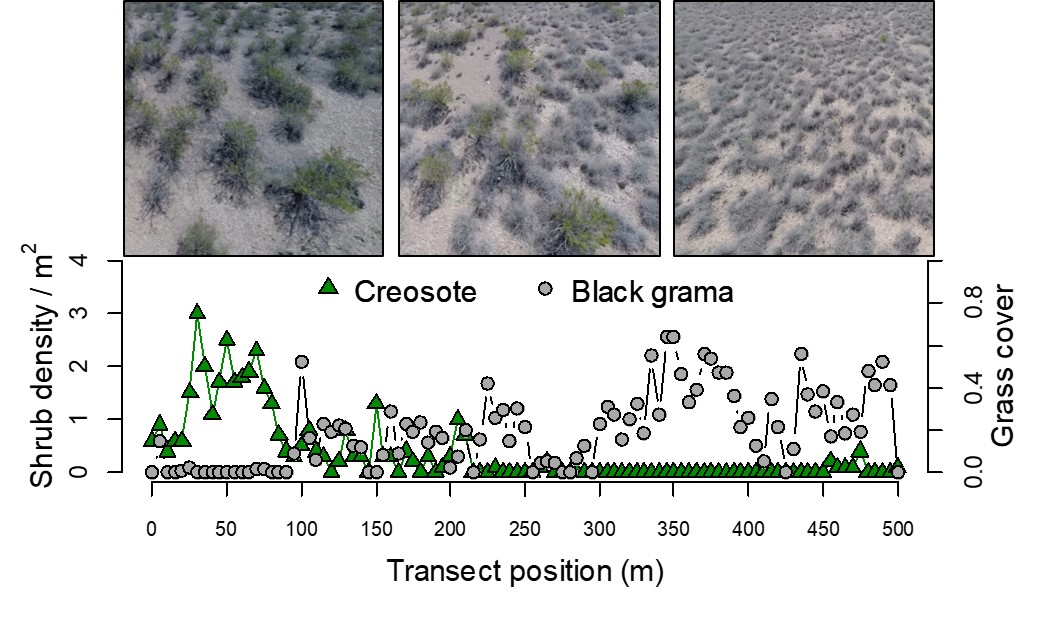
\includegraphics[width=\linewidth]{Figures/waves_pics}
    \caption{}
  \label{fig:waves}
  \end{center}
\end{figure}

\newpage
\begin{figure}[H]
  \begin{center}
    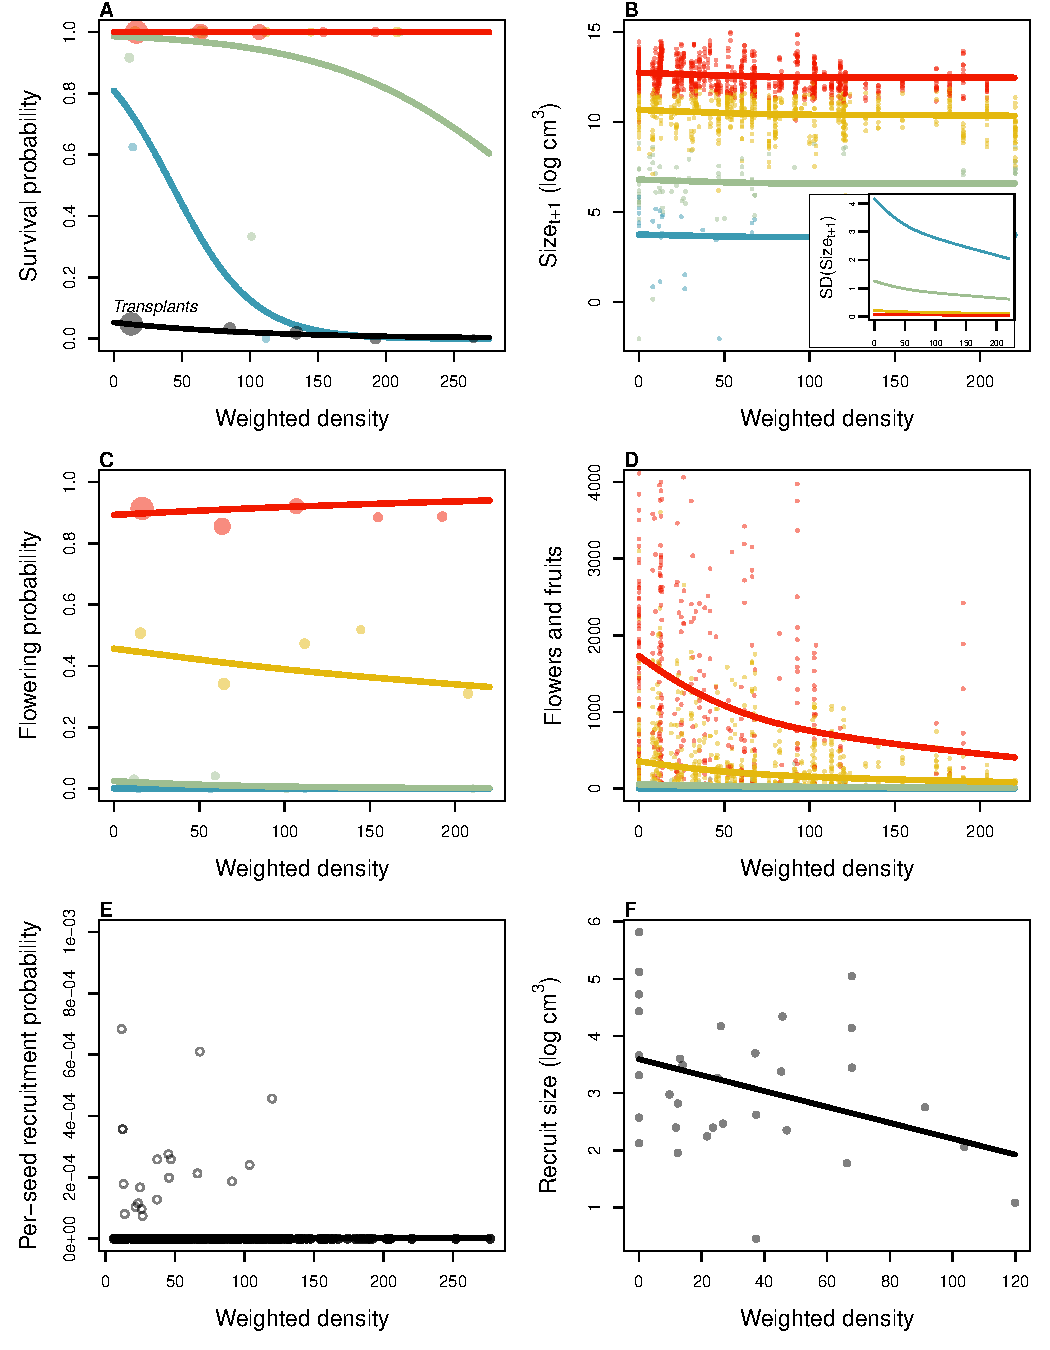
\includegraphics[width=\linewidth]{Figures/vital_rates}
  \caption{}
  \label{fig:vital_rates}
  \end{center}
\end{figure}

\newpage
\begin{figure}[H]
  \begin{center}
    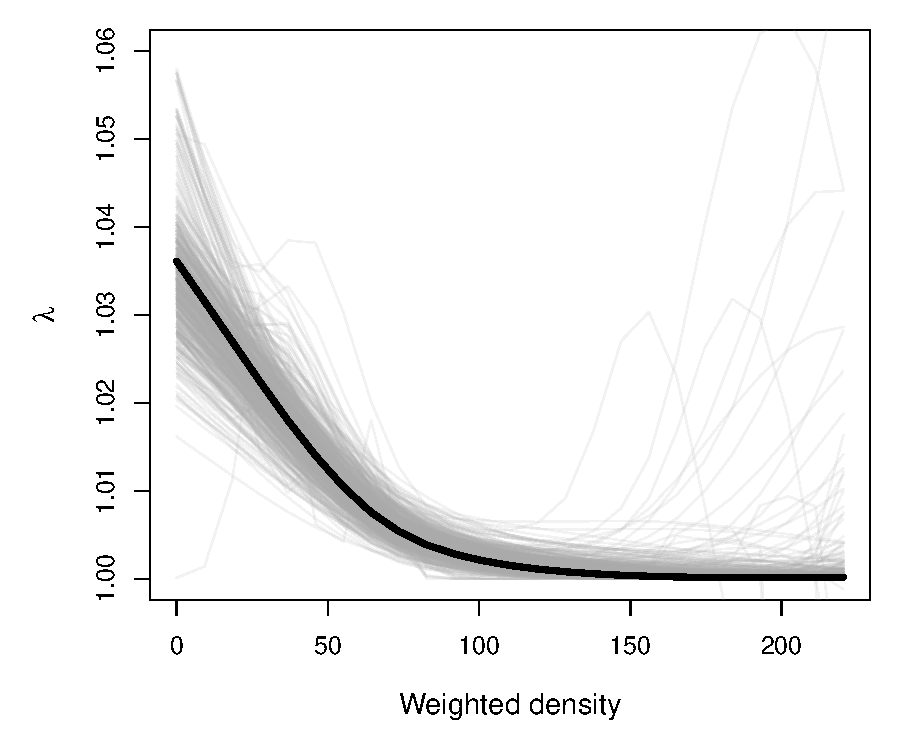
\includegraphics[width=\linewidth]{Figures/LambdaD}
  \caption{}
  \label{fig:lambda}
  \end{center}
\end{figure}

\newpage
\begin{figure}[H]
  \begin{center}
    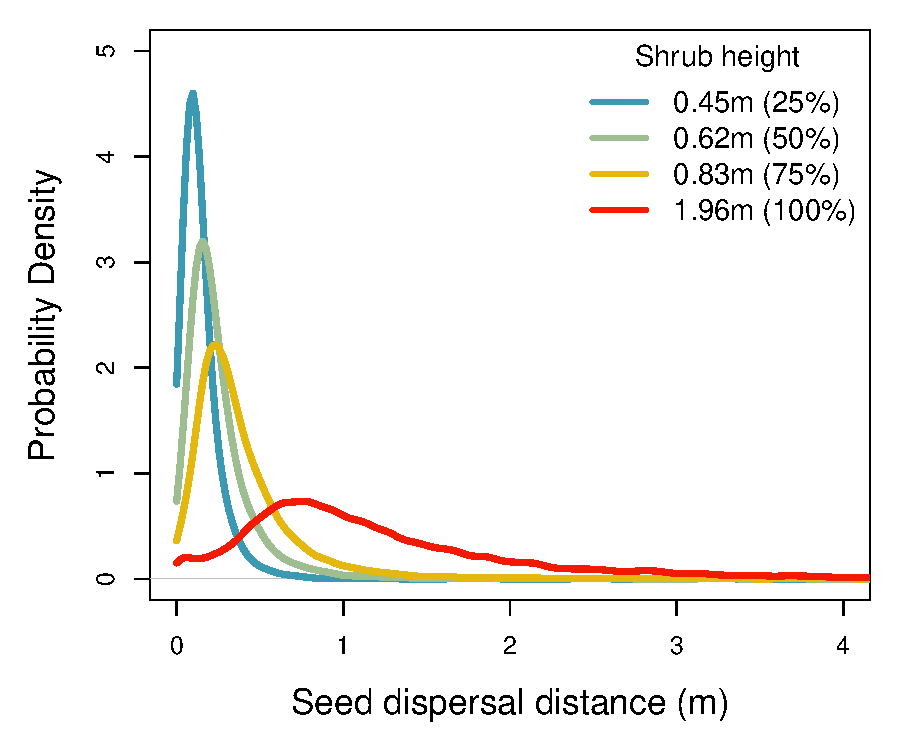
\includegraphics[width=\linewidth]{Figures/Dkernels}
  \caption{}
  \label{fig:dispersal}
  \end{center}
\end{figure}

\newpage
\begin{figure}[H]
  \begin{center}
    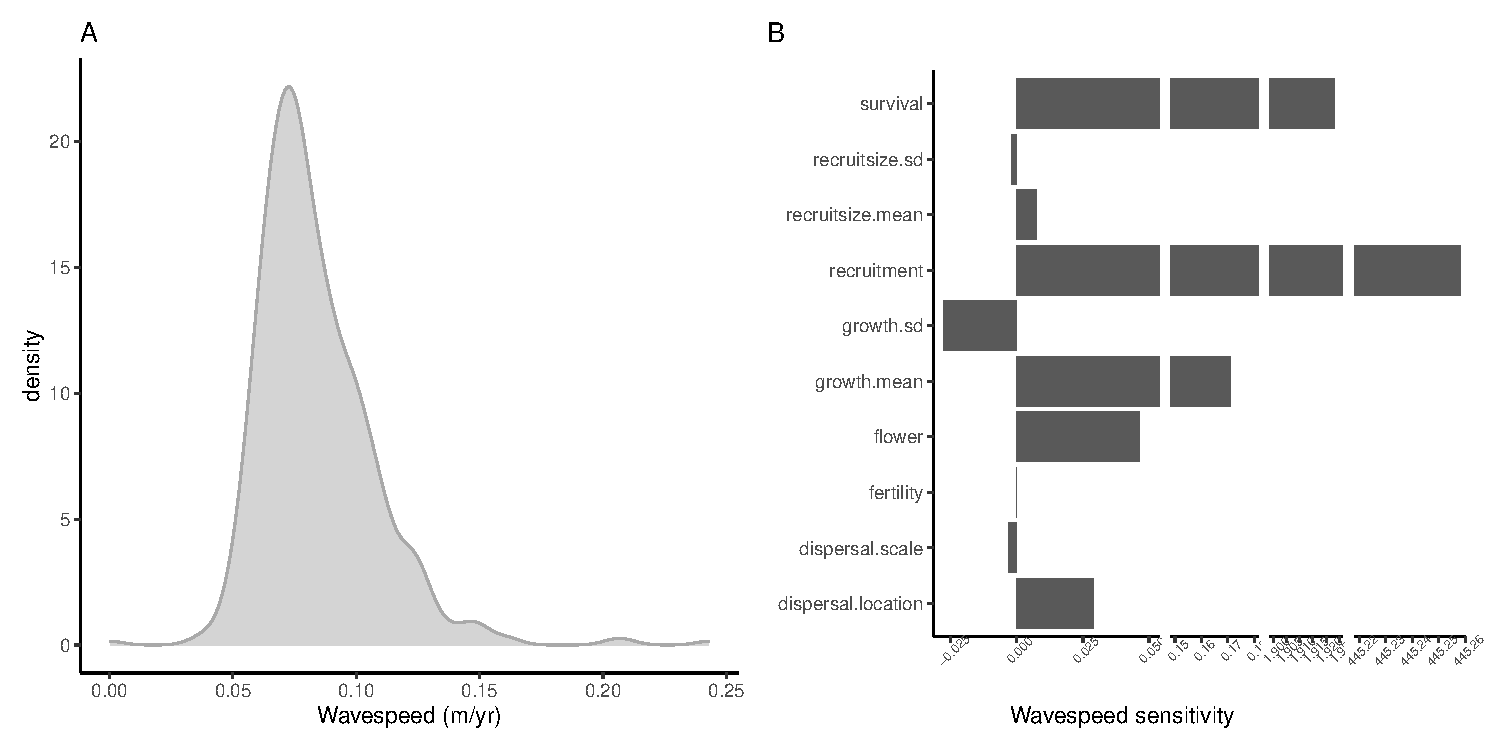
\includegraphics[width=\linewidth]{Figures/wavespeed_sens}
  \caption{}
  \label{fig:wavespeed}
  \end{center}
\end{figure}

\newpage
\begin{figure}[H]
  \begin{center}
    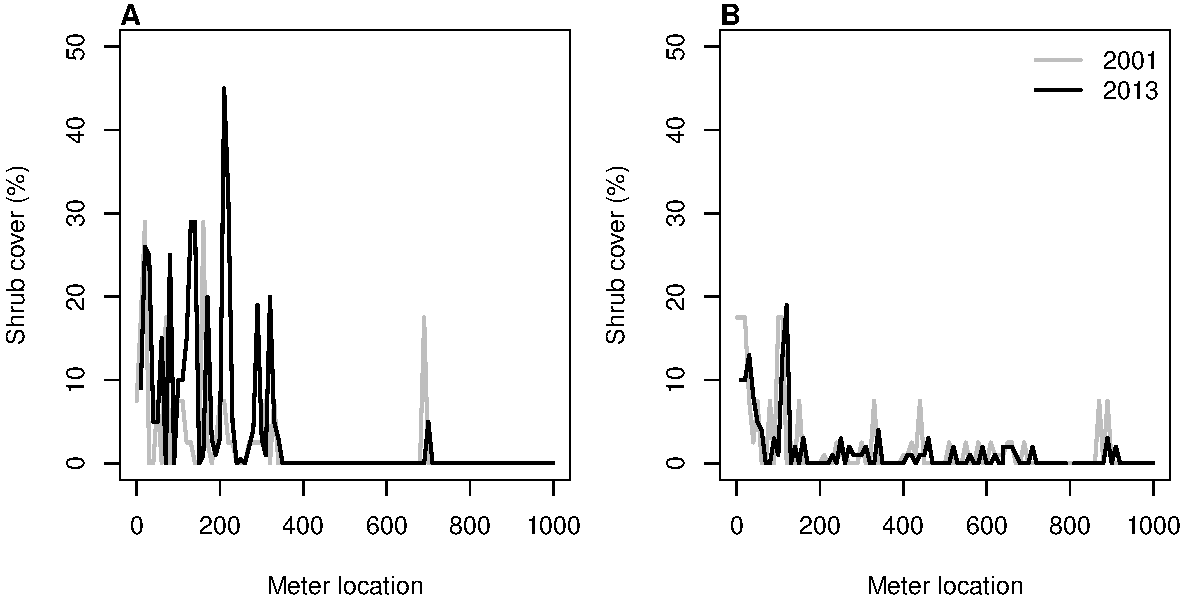
\includegraphics[width=\linewidth]{Figures/resurveys}
  \caption{}
  \label{fig:resurvey}
  \end{center}
\end{figure}

\newpage
\section*{Appendix A: Dispersal kernel modeling}
\renewcommand{\thefigure}{A\arabic{figure}}\setcounter{figure}{0}
\renewcommand{\thetable}{A\arabic{table}}\setcounter{table}{0}
\renewcommand{\theequation}{A\arabic{equation}}\setcounter{equation}{0}

\paragraph{WALD dispersal kernel}
In order to create the dispersal kernel, we first take the wind speeds at measurement height $z_{m}$ and correct them to find wind speed $U$ for any height $H$ by using the logarithmic wind profile

\begin{linenomath*} \begin{equation} U = \frac{1}{H} \int_{d+z_{0}}^{H} \frac{u^*}{K} \log \left(\frac{z-d}{z_{0}}\right) dz \end{equation} 
\end{linenomath*} 

given in \citet{bullock2012modelling} equation 6, with the notation slightly modified. 
Here, $z$ is the height above the ground, $K$ is the von Karman constant, and $u^*$ is the friction velocity.
The zero-plane displacement $d$ and roughness length $z_{0}$ are surface roughness parameters that, for a grass canopy height $h$ above the ground, are  approximated by $d \approx 0.7h$ and $z_{0} \approx 0.1h$.
These estimates are from \citet{raupach1994simplified} for a canopy area index $\Lambda = 1$ in which the sum of grass canopy elements is equal to the unit area being measured.
A 0.15 m grass height at our study site gives $d = 0.105$ and $z_{0} = 0.015$, which are suitable approximations for grassland \citep{wiernga1993representative}.
Calculations of $u^*$ were done using equation A2 from \citet{skarpaas2007dispersal}, in which 

\begin{linenomath*} \begin{equation} u^* = KU_{m} \left[\log\left(\frac{z_{m} - d}{z_{0}}\right)\right]^{-1} \end{equation} 
\end{linenomath*} 

and $U_{m}$ is the mean wind velocity at the measurement height $z_{m}$.
Values for the turbulent flow parameter $\sigma$ were then calculated using the estimate made by \citet{skarpaas2007dispersal} in their equation A4, where 

\begin{linenomath*} \begin{equation} \sigma = 2A_{w}^2 \sqrt{\frac{K(z-d)u^*}{C_{0}U}} \end{equation} 
\end{linenomath*} 

and $C_{0}$ is the Kolmogorov constant.
$A_{w}$ is a constant that relates vertical turbulence to friction velocity and is approximately equal to 1.3 under the assumptions of above-canopy flow made by \citet{skarpaas2007dispersal}, based off calculations from \citet{hsieh1997dissipation}.
We used maximum plant height $H$ as a measure of $z$.

The values from the previous three equations give us the necessary information to calculate $\mu'$ and $\lambda'$, thus allowing us to create the WALD distribution $p(r)$.
However, the base WALD model does not take into account variation in wind speeds or seed terminal velocities, which limits its applicability in systems where such variation is present.
In order to account for this variation, we integrate the WALD model over distributions of these two variables using the same method as \citet{skarpaas2007dispersal}.
Additionally, the WALD model assumes seed release from a single point source, which is not realistic for creosotebush; because seeds are released across the entire height of the shrub rather than from a point source, we integrated $p(r)$ across the uniform distribution from the grass canopy height to the shrub height.
Thus, under the assumptions that the height at which a seed is located does not affect its probability of being released and that seeds are evenly distributed throughout the shrub, this gives the dispersal kernel $K(r)$, where

\begin{linenomath*} \begin{equation} K(r) = \iiint p(F)p(U)p(z)p(r) \,dF\,dU\,dz \end{equation} 
\end{linenomath*} 

and $p(F)$ and $p(U)$ are the PDFs of the terminal velocity $F$ and wind speed $U$, respectively, and $p(z)$ is the uniform distribution from $h$ to $H$.

\paragraph{Dispersal data collection}
The distribution $p(F)$ in the integral above was constructed using experimentally determined seed terminal velocities.
These velocities were estimated using laboratory-based seed release experiments with a high-speed camera and motion tracking software to determine position as a function of time.
We then used the Levenberg-Marquardt algorithm to solve a quadratic-drag equation of motion for $F$. 
Before seeds were released, they were dried, dyed with yellow fluorescent powder, and then put against a black background to improve visibility and make tracking easier.
While the powder added mass to the seeds, this added mass only yielded an approximately 2.5\% increase, likely having little effect on terminal velocities.
Measurements were conducted for 48 seeds that were randomly chosen from a seed pool derived from different plants, and then an empirical PDF of terminal velocities was constructed using the data.
Constructing $p(U)$ involved creating an empirical PDF of hourly wind speeds using data from Sevilleta LTER meterological station 49, the station closest to our transects.
We used wind speed data collected hourly from 2015 to 2019 \citep{SEVmet}.

\newpage
\section*{Appendix B: Additional results}
\renewcommand{\thefigure}{B\arabic{figure}}\setcounter{figure}{0}
\renewcommand{\thetable}{B\arabic{table}}\setcounter{table}{0}
\renewcommand{\theequation}{B\arabic{equation}}\setcounter{equation}{0}

% latex table generated in R 4.2.0 by xtable 1.8-4 package
% Wed Oct  5 09:35:25 2022
\begin{table}[ht]
\centering
\begin{tabular}{|p{12cm}|c|c|}
  \hline
Pr(Survival) & df & dAIC \\ 
  \hline
\~{}size + transplant + size:transplant + (1$|$transect) & 11.50 & 1.72 \\ 
  \~{}size + transplant + density + size:transplant + density:transplant + (1$|$transect) & 13.19 & 0.19 \\ 
  \~{}size + transplant + density + size:transplant + density:transplant + size:density + size:transplant:density + (1$|$transect) & 14.22 & 0.00 \\ 
   \hline
\end{tabular}
\caption{AIC model selection for survival probability.} 
\label{tab:surv_aic}
\end{table}


% latex table generated in R 4.2.0 by xtable 1.8-4 package
% Wed Oct  5 09:35:25 2022
\begin{table}[ht]
\centering
\begin{tabular}{|p{8cm}|p{4cm}|c|c|}
  \hline
mean(size) & sd(size) & df & dAIC \\ 
  \hline
\~{}size + (1$|$transect) & \~{}1 & 3.00 & 1024.88 \\ 
  \~{}size + density + (1$|$transect) & \~{}1 & 8.50 & 977.23 \\ 
  \~{}size + density + size:density + (1$|$transect) & \~{}1 & 10.47 & 975.17 \\ 
  \~{}size + (1$|$transect) & \~{}size & 9.65 & 146.23 \\ 
  \~{}size + density + (1$|$transect) & \~{}size & 16.24 & 19.45 \\ 
  \~{}size + density + size:density + (1$|$transect) & \~{}size & 18.55 & 19.62 \\ 
  \~{}size + (1$|$transect) & \~{}size + density & 10.40 & 115.52 \\ 
  \~{}size + density + (1$|$transect) & \~{}size + density & 18.97 & 0.08 \\ 
  \~{}size + density + size:density + (1$|$transect) & \~{}size + density & 21.33 & 0.00 \\ 
   \hline
\end{tabular}
\caption{AIC model selection for mean and variance of future size} 
\label{tab:grow_aic}
\end{table}



% latex table generated in R 4.2.0 by xtable 1.8-4 package
% Wed Oct  5 09:35:25 2022
\begin{table}[ht]
\centering
\begin{tabular}{|p{8cm}|c|c|}
  \hline
Pr(Flowering) & df & dAIC \\ 
  \hline
\~{}size + (1$|$transect) & 5.78 & 0.63 \\ 
  \~{}size + density + (1$|$transect) & 6.80 & 2.32 \\ 
  \~{}size + density + size:density + (1$|$transect) & 7.24 & 0.00 \\ 
   \hline
\end{tabular}
\caption{AIC model selection for flowering probability.} 
\label{tab:flow_aic}
\end{table}



% latex table generated in R 4.2.0 by xtable 1.8-4 package
% Wed Oct  5 09:35:25 2022
\begin{table}[ht]
\centering
\begin{tabular}{|p{8cm}|c|c|}
  \hline
No. fruits & df & dAIC \\ 
  \hline
\~{}size + (1$|$transect) & 14.25 & 71.99 \\ 
  \~{}size + density + (1$|$transect) & 5.52 & 0.00 \\ 
  \~{}size + density + size:density + (1$|$transect) & 6.23 & 0.37 \\ 
   \hline
\end{tabular}
\caption{AIC model selection for fruit number.} 
\label{tab:fruit_aic}
\end{table}


% latex table generated in R 4.2.0 by xtable 1.8-4 package
% Wed Oct  5 09:35:25 2022
\begin{table}[ht]
\centering
\begin{tabular}{|p{8cm}|c|c|}
  \hline
Pr(Recruitment) & df & dAIC \\ 
  \hline
\~{}(1$|$transect) & 6.57 & 0.00 \\ 
  \~{}density + (1$|$transect) & 7.39 & 0.93 \\ 
   \hline
\end{tabular}
\caption{AIC model selection for recruitment probability.} 
\label{tab:recruit_aic}
\end{table}


% latex table generated in R 4.2.0 by xtable 1.8-4 package
% Wed Oct  5 09:35:25 2022
\begin{table}[ht]
\centering
\begin{tabular}{|p{8cm}|p{4cm}|c|c|}
  \hline
mean(size) & sd(size) & df & dAIC \\ 
  \hline
\~{}(1$|$transect) & \~{}1 & 2.00 & 2.90 \\ 
  \~{}density+(1$|$transect) & \~{}1 & 4.42 & 0.00 \\ 
  \~{}(1$|$transect) & \~{}density & 3.00 & 4.74 \\ 
  \~{}density+(1$|$transect) & \~{}density & 5.56 & 1.21 \\ 
   \hline
\end{tabular}
\caption{AIC model selection for mean and variance of recruit size.} 
\label{tab:recruitsize_aic}
\end{table}


\newpage
\begin{figure}[H]
  \begin{center}
    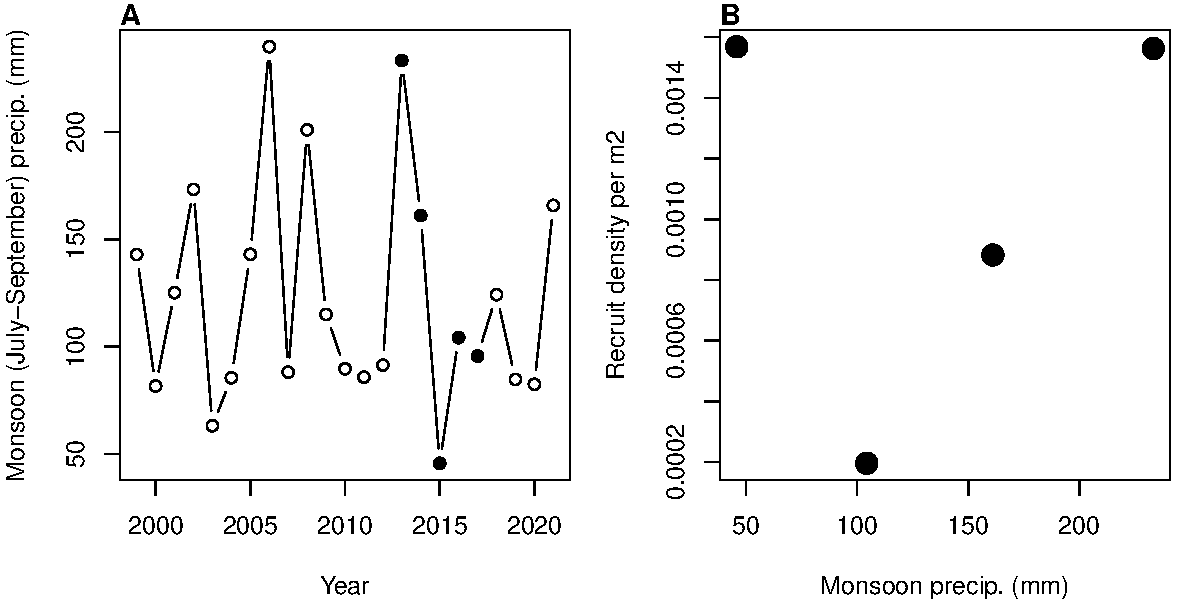
\includegraphics[width=\linewidth]{Figures/monsoon_seedlings}
  \caption{A, Time series of annual monsoon precipitation (filled circles are the years in which this study was conducted). B, Relationship between density of creosotebush recruits observed on our transects in May-June and monsoon precipitation in the preceding July-September.}
  \label{fig:monsoon}
  \end{center}
\end{figure}

\newpage
\section*{Appendix C: Additional transplant analysis}
\renewcommand{\thefigure}{C\arabic{figure}}\setcounter{figure}{0}
\renewcommand{\thetable}{C\arabic{table}}\setcounter{table}{0}
\renewcommand{\theequation}{C\arabic{equation}}\setcounter{equation}{0}

We censused transplant survival twice following July 2015 planting, in fall 2015 and spring 2016. 
Here, we analyze the two survival intervals separately, including grass and shrub cover at the local ($1m$x$1m$) scale as explanatory variables in addition to the weighted density of the 5-m transect window as presented in the main text. 

For both fall and spring survival censuses, we fit eight candidate models that included all combinations of window weighted density, local shrub cover (proportion of plot area covered by creosotebush), and local grass cover (proportion of plot area covered by any grass species) as smooth terms in a generalized additive model.
We used a binomial response distribution where ``successes'' were the number of survivors per plot and ``trials'' were the number of seedlings planted for fall survival (always four per plot) and the number of fall survivors for spring survival. 
All models included a random effect of transect. 
We used AIC-based model selection to quantify support for competing models. 

\paragraph{Results}The majority of mortality occurred within the first census interval (53 fall survivors out of 576 transplants), resulting in a much smaller data set for the second census interval (20 spring survivors out of 53 fall survivors).

For fall survival, the top model (Model 7) included effects of creosotebush weighted density at the 5-m window scale and local grass cover (Table \ref{tab:fall_aic}). 
Fall survival was low overall but greatest in zero-density windows and there was a weak negative effect of local grass cover (Figure \ref{fig:survapp}).
Three additional models (2, 5 and 8) were within 2 AIC units of the top model (Table \ref{tab:fall_aic}). 
Despite the model uncertainty, these top four models included shrub weighted density and comprised \>87\% of AIC weight, providing strong support for negative effects of shrub density at the scale of 5-m windows, consistent with the full analysis (transplant experiment + observational census) presented in the main text.

Spring survival was dominated by high model uncertainty, and the most complex model (8) did not converge due to inadequate data. 
The top-ranked model was Model 6, which included effects of local shrub and grass cover.
However, the null model (1) was nearly tied with the top model, and six of seven models were within 2 AIC units. 
Given the relatively small data set, a conservative interpretation is that there is not sufficient evidence to reject the null hypothesis of a constant fall-to-spring survival rate that was unrelated to shrub or grass density. 

% latex table generated in R 4.2.0 by xtable 1.8-4 package
% Wed Oct  5 09:35:25 2022
\begin{table}[ht]
\centering
\begin{tabular}{|p{12cm}|c|c|}
  \hline
Pr(Survival) & df & dAIC \\ 
  \hline
(1$|$transect) & 8.93 & 11.98 \\ 
  window density + (1$|$transect) & 9.97 & 0.49 \\ 
  shrub cover + (1$|$transect) & 10.82 & 3.51 \\ 
  grass cover + (1$|$transect) & 11.02 & 6.65 \\ 
  window density + shrub cover + (1$|$transect) & 12.11 & 1.04 \\ 
  grass cover + shrub cover + (1$|$transect) & 12.29 & 3.29 \\ 
  window density + grass cover + (1$|$transect) & 11.44 & 0.00 \\ 
  window density + shrub cover + grass cover + (1$|$transect) & 12.39 & 1.80 \\ 
   \hline
\end{tabular}
\caption{AIC model selection for July-October transplant survival probability.} 
\label{tab:fall_aic}
\end{table}


% latex table generated in R 4.2.0 by xtable 1.8-4 package
% Wed Oct  5 09:35:25 2022
\begin{table}[ht]
\centering
\begin{tabular}{|p{12cm}|c|c|}
  \hline
Pr(Survival) & df & dAIC \\ 
  \hline
(1$|$transect) & 1.00 & 0.07 \\ 
  window density + (1$|$transect) & 2.00 & 1.93 \\ 
  shrub cover + (1$|$transect) & 2.00 & 1.22 \\ 
  grass cover + (1$|$transect) & 2.03 & 0.69 \\ 
  window density + shrub cover + (1$|$transect) & 3.00 & 1.85 \\ 
  grass cover + shrub cover + (1$|$transect) & 3.37 & 0.00 \\ 
  window density + grass cover + (1$|$transect) & 3.23 & 2.19 \\ 
   \hline
\end{tabular}
\caption{AIC model selection for October-June transplant survival probability.} 
\label{tab:spring_aic}
\end{table}


\begin{figure}[H]
  \begin{center}
    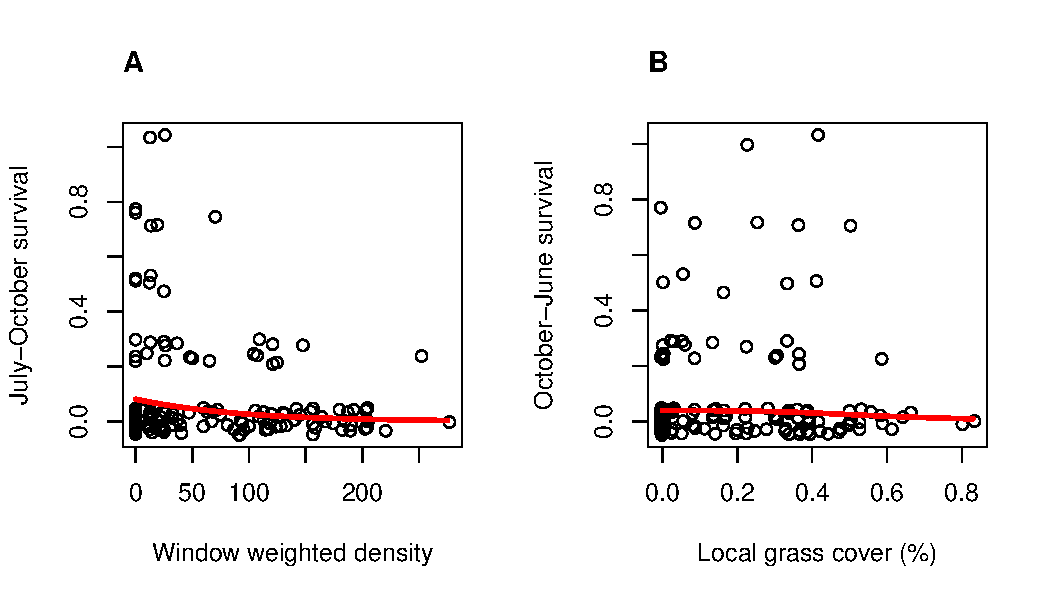
\includegraphics[width=\linewidth]{Figures/survival_appendix}
  \caption{}
  \label{fig:survapp}
  \end{center}
\end{figure}

\end{document}
